% !TeX root = ../../tesi.tex

Neural networks (NNs) are parametric function approximators inspired by the distributed information-processing paradigm of biological nervous systems. At a conceptual level, an NN is composed of interconnected layers of artificial neurons, where each neuron receives a set of inputs, combines them linearly through trainable weights and biases, and then applies a non-linear activation function. By stacking multiple layers, the network implements a nested composition of transformations that can model highly non-linear input--output relationships \cite{goodfellow_deep_2016}. During training, the parameters are adjusted so as to minimize a task-specific loss function, thereby enabling the network to progressively improve its predictions from data \cite{goodfellow_deep_2016}.

\begin{figure}[h]
    \centering
    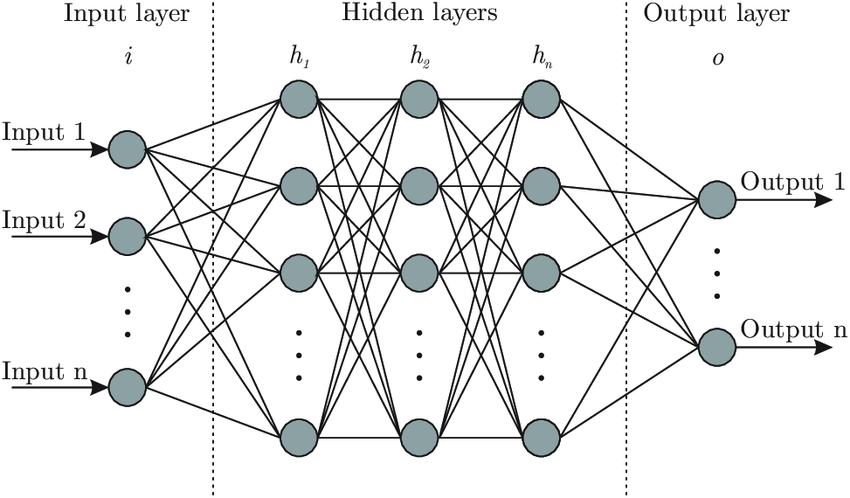
\includegraphics[width=0.5\textwidth]{images/NN.png}
    \caption{Schematic representation of a feedforward neural network with multiple hidden layers. Each layer applies a linear transformation followed by a non-linear activation, enabling progressively richer representations of the input.}
\end{figure}

The optimization of neural networks is typically performed through \textbf{gradient descent} and its stochastic variants. After computing the loss associated with a prediction, gradient descent updates the model parameters in the direction that most reduces the loss, with the size of each update controlled by the learning rate. Backpropagation provides the mechanism that makes this process computationally feasible: by applying the chain rule from the output layer back to the earlier layers, it efficiently computes the gradient of the loss with respect to each parameter in the network \cite{rumelhart_learning_1986,goodfellow_deep_2016}. Together, gradient-based optimization and backpropagation allow neural networks to learn complex functions directly from data.

\begin{figure}[h]
    \centering
    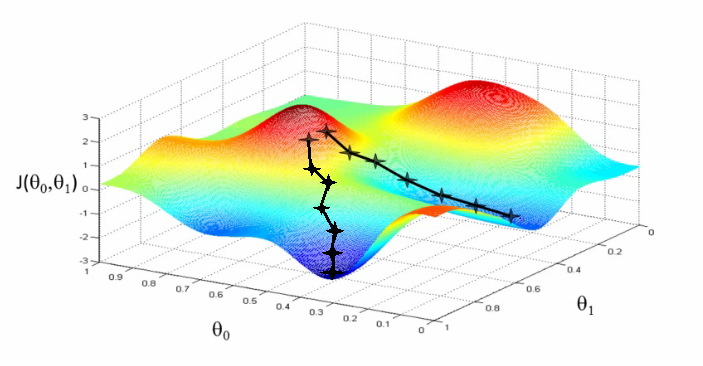
\includegraphics[width=0.5\textwidth]{images/Gradient_descent.png}
    \caption{Illustration of gradient descent over a loss surface. At each iteration, the parameters are updated in the direction of the negative gradient so as to reduce the loss.}
\end{figure}

\subsection{Deep Learning}
While the term neural network refers broadly to a family of trainable models composed of interconnected artificial neurons, \textbf{deep learning} denotes the specific setting in which these models contain multiple representation-learning layers arranged in depth \cite{goodfellow_deep_2016}. The practical importance of depth lies in its ability to learn hierarchical representations: lower layers tend to encode simpler patterns, whereas deeper layers combine them into progressively more abstract and task-relevant features \cite{lecun_deep_2015,goodfellow_deep_2016}. This property distinguishes deep learning from earlier machine learning pipelines, in which feature extraction was often designed manually before classification or regression.

By making end-to-end representation learning possible, deep learning allows the model to infer useful features directly from raw or weakly processed data rather than relying on handcrafted descriptors \cite{goodfellow_deep_2016}. This shift has been one of the main reasons for the remarkable progress observed across computer vision, speech, and natural language processing. At the same time, the high representational capacity of deep models generally \textbf{requires large datasets}, substantial computational resources, and careful optimization procedures in order to achieve strong generalization performance \cite{lecun_deep_2015}. A decisive milestone in this development was the success of deep convolutional networks in large-scale visual recognition, which accelerated both scientific interest and industrial adoption \cite{krizhevsky_imagenet_2012}.
\begin{figure}[h]
    \centering
    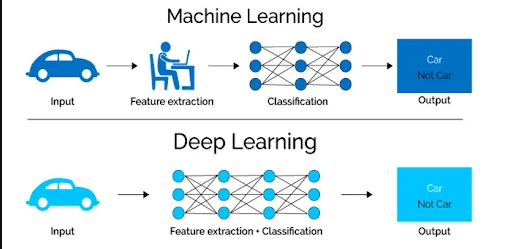
\includegraphics[width=0.5\textwidth]{images/DL.png}
    \caption{Schematic representation of a deep neural network, where feature representations are learned across multiple layers of abstraction and not manually engineered.}
\end{figure}

\subsection{Convolutional Neural Networks}
Among deep architectures for visual data, \textbf{Convolutional Neural Networks (CNNs)} have long represented the dominant paradigm. Their design is based on local receptive fields, \textbf{shared convolutional kernels}, and hierarchical feature extraction as for deep learning nets, which introduce useful inductive biases such as translation equivariance and improved parameter efficiency \cite{lecun_gradient-based_1998,goodfellow_deep_2016}. In a convolutional layer, the same learnable kernel is applied across different spatial positions of the input image, producing feature maps that respond to recurring \textbf{local patterns}. This combination of local connectivity and parameter sharing drastically reduces the number of trainable parameters, making CNNs more efficient to optimize and, in many practical settings, less data-hungry than generic dense architectures for visual tasks \cite{goodfellow_deep_2016,lecun_gradient-based_1998}. 

The use of kernels is particularly well suited to images because relevant visual structures, such as edges, corners, textures, and simple shapes, are inherently local. By learning detectors for these local patterns and reusing them across the whole image, CNNs can extract meaningful features while preserving spatial structure. This property generally improves generalization to unseen images and makes CNNs effective even when computational resources or dataset sizes are more limited than those required by less structured architectures \cite{goodfellow_deep_2016,lecun_gradient-based_1998}. In practice, early layers tend to capture low-level structures, whereas deeper layers encode increasingly abstract semantic patterns. Additional operations such as spatial downsampling or pooling further enlarge the effective receptive field and support the progressive aggregation of information across layers \cite{lecun_gradient-based_1998}. This hierarchical organization explains the effectiveness of CNNs in tasks such as image classification, object detection, and semantic segmentation.

\begin{figure}[h]
    \centering
    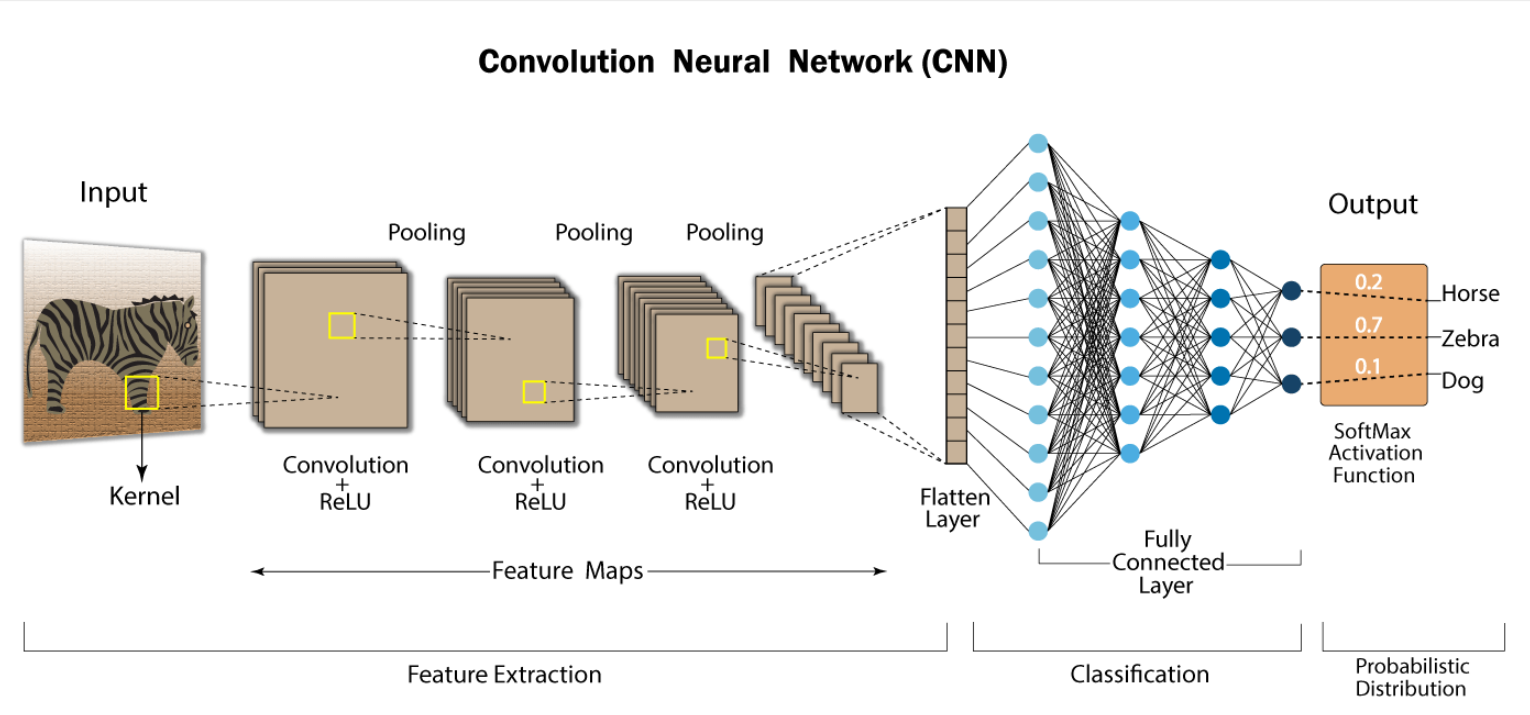
\includegraphics[width=0.52\textwidth]{images/CNN.png}
    \caption{Typical convolutional neural network architecture for visual processing, in which convolutional and downsampling stages progressively extract hierarchical features from the input image.}
\end{figure}

In the context of this thesis, neural networks, deep learning, and CNNs provide the conceptual foundation for the architectures discussed in the following sections. Vision Transformers and RT-DETR will therefore be introduced as successive developments built upon, or reacting to, this baseline \cite{dosovitskiy_image_2021,zhao_detrs_2024}.
